% Options for packages loaded elsewhere
\PassOptionsToPackage{unicode}{hyperref}
\PassOptionsToPackage{hyphens}{url}
%
\documentclass[
]{article}
\usepackage{amsmath,amssymb}
\usepackage{lmodern}
\usepackage{iftex}
\ifPDFTeX
  \usepackage[T1]{fontenc}
  \usepackage[utf8]{inputenc}
  \usepackage{textcomp} % provide euro and other symbols
\else % if luatex or xetex
  \usepackage{unicode-math}
  \defaultfontfeatures{Scale=MatchLowercase}
  \defaultfontfeatures[\rmfamily]{Ligatures=TeX,Scale=1}
\fi
% Use upquote if available, for straight quotes in verbatim environments
\IfFileExists{upquote.sty}{\usepackage{upquote}}{}
\IfFileExists{microtype.sty}{% use microtype if available
  \usepackage[]{microtype}
  \UseMicrotypeSet[protrusion]{basicmath} % disable protrusion for tt fonts
}{}
\makeatletter
\@ifundefined{KOMAClassName}{% if non-KOMA class
  \IfFileExists{parskip.sty}{%
    \usepackage{parskip}
  }{% else
    \setlength{\parindent}{0pt}
    \setlength{\parskip}{6pt plus 2pt minus 1pt}}
}{% if KOMA class
  \KOMAoptions{parskip=half}}
\makeatother
\usepackage{xcolor}
\usepackage[margin=1in]{geometry}
\usepackage{graphicx}
\makeatletter
\def\maxwidth{\ifdim\Gin@nat@width>\linewidth\linewidth\else\Gin@nat@width\fi}
\def\maxheight{\ifdim\Gin@nat@height>\textheight\textheight\else\Gin@nat@height\fi}
\makeatother
% Scale images if necessary, so that they will not overflow the page
% margins by default, and it is still possible to overwrite the defaults
% using explicit options in \includegraphics[width, height, ...]{}
\setkeys{Gin}{width=\maxwidth,height=\maxheight,keepaspectratio}
% Set default figure placement to htbp
\makeatletter
\def\fps@figure{htbp}
\makeatother
\setlength{\emergencystretch}{3em} % prevent overfull lines
\providecommand{\tightlist}{%
  \setlength{\itemsep}{0pt}\setlength{\parskip}{0pt}}
\setcounter{secnumdepth}{-\maxdimen} % remove section numbering
\ifLuaTeX
  \usepackage{selnolig}  % disable illegal ligatures
\fi
\IfFileExists{bookmark.sty}{\usepackage{bookmark}}{\usepackage{hyperref}}
\IfFileExists{xurl.sty}{\usepackage{xurl}}{} % add URL line breaks if available
\urlstyle{same} % disable monospaced font for URLs
\hypersetup{
  pdftitle={final project},
  pdfauthor={Haokun Zhang, Zhang Lu, Jonathan},
  hidelinks,
  pdfcreator={LaTeX via pandoc}}

\title{final project}
\author{Haokun Zhang, Zhang Lu, Jonathan}
\date{2023-04-20}

\begin{document}
\maketitle

\hypertarget{workflow}{%
\subsubsection{Workflow}\label{workflow}}

\hypertarget{define-the-question-how-much-should-we-pay-for-audit-fee}{%
\subsubsection{1. Define the question: How much should we pay for Audit
fee?}\label{define-the-question-how-much-should-we-pay-for-audit-fee}}

\hypertarget{data-wranglingcompleted}{%
\subsubsection{2. Data
wrangling(Completed)}\label{data-wranglingcompleted}}

\hypertarget{data-visualizationeda---exploratory-data-analysis}{%
\subsubsection{3. Data Visualization(EDA - Exploratory Data
Analysis)}\label{data-visualizationeda---exploratory-data-analysis}}

\hypertarget{unsupervised-learning-use-pcamix-and-k-means-clustering-to-do-the-company-segmentation-like-ux7e7cux9d6cux4ed6ux5011ux505aux7684}{%
\subsubsection{4. Unsupervised learning: Use PCAmix and K-means++
clustering to do the company segmentation? Like
繼鵬他們做的)}\label{unsupervised-learning-use-pcamix-and-k-means-clustering-to-do-the-company-segmentation-like-ux7e7cux9d6cux4ed6ux5011ux505aux7684}}

\hypertarget{then-choose-the-modelsupervised-learning}{%
\subsubsection{Then choose the model(Supervised
learning):}\label{then-choose-the-modelsupervised-learning}}

\hypertarget{linear-regression-knn-regression-tree-random-forest-cart-boosting-lasso-regression}{%
\subsubsection{Linear regression, knn, Regression tree: random forest,
CART, Boosting \& Lasso
regression}\label{linear-regression-knn-regression-tree-random-forest-cart-boosting-lasso-regression}}

\hypertarget{ux5b78ux7e7cux9d6cux7528lasso-ux548crandom-forestux5169ux500bmodelux627eux51faux6703ux5f71ux97ffaudit-feeux7684ux56e0ux7d20ux6709ux54eaux4e9b}{%
\subsubsection{5. 學繼鵬:用lasso 和Random
Forest兩個model,找出會影響audit
fee的因素有哪些}\label{ux5b78ux7e7cux9d6cux7528lasso-ux548crandom-forestux5169ux500bmodelux627eux51faux6703ux5f71ux97ffaudit-feeux7684ux56e0ux7d20ux6709ux54eaux4e9b}}

\hypertarget{model-training-split-to-training-set-testing-set-do-the-k-fold-cross-validation}{%
\subsubsection{6. Model training: Split to Training set \& Testing set,
do the K-fold
Cross-Validation}\label{model-training-split-to-training-set-testing-set-do-the-k-fold-cross-validation}}

\hypertarget{assess-the-model-performance-k-fold-cv-mse-r-square-f-1-scorethe-chart-of-actual-and-predicted}{%
\subsubsection{7. Assess the model performance: k-fold cv, MSE,
R-square, F-1 score(the chart of actual and
predicted)}\label{assess-the-model-performance-k-fold-cv-mse-r-square-f-1-scorethe-chart-of-actual-and-predicted}}

\hypertarget{choose-the-best-performance-modeluse-it-to-do-the-predictionux4e26ux4e14ux5c07ux7d50ux679cux5716ux8868ux5316-partial-dependence-plots-etc}{%
\subsubsection{( Choose the best performance model,use it to do the
prediction,並且將結果圖表化? Partial dependence plots
etc)}\label{choose-the-best-performance-modeluse-it-to-do-the-predictionux4e26ux4e14ux5c07ux7d50ux679cux5716ux8868ux5316-partial-dependence-plots-etc}}

\hypertarget{conclusion-what-did-we-learn--ux6839ux64daux4e0dux540cux7684input-value-ux53efux4ee5ux9810ux6e2caudit-feeux70baux591aux5c11}{%
\subsubsection{8. Conclusion: What did we learn- 根據不同的input value,
可以預測audit
fee為多少}\label{conclusion-what-did-we-learn--ux6839ux64daux4e0dux540cux7684input-value-ux53efux4ee5ux9810ux6e2caudit-feeux70baux591aux5c11}}

\hypertarget{workflow-if-learn-from-other-ppl}{%
\subsubsection{Workflow if learn from other
ppl}\label{workflow-if-learn-from-other-ppl}}

\hypertarget{same}{%
\subsubsection{1\textasciitilde4 same}\label{same}}

\hypertarget{use-lasso-regression-and-do-th-cv-find-the-important-coefficientsmore-robust-and-understandable-coefficients}{%
\subsubsection{5. Use lasso regression and do th cv, find the important
coefficients(more robust and understandable
coefficients)}\label{use-lasso-regression-and-do-th-cv-find-the-important-coefficientsmore-robust-and-understandable-coefficients}}

\hypertarget{use-random-forest-to-measure-the-variable-importancebetter-fit-but-less-interpretability-and-use-partial-plots}{%
\subsubsection{6. Use Random Forest to measure the variable
importance(better fit but less interpretability), and use partial
plots}\label{use-random-forest-to-measure-the-variable-importancebetter-fit-but-less-interpretability-and-use-partial-plots}}

\hypertarget{end}{%
\subsubsection{End}\label{end}}

\hypertarget{problem-zone}{%
\subsection{Problem zone}\label{problem-zone}}

\hypertarget{how-to-assess-the-model-performance-bc-lasso-model-ux597dux50cfux4e0dux80fdux7528mseux53bbux8a55ux50f9-if-not-what-can-we-use-to-assess-the-model}{%
\subsubsection{1. How to assess the model performance? BC Lasso model
好像不能用MSE去評價? If not, what can we use to assess the
model?}\label{how-to-assess-the-model-performance-bc-lasso-model-ux597dux50cfux4e0dux80fdux7528mseux53bbux8a55ux50f9-if-not-what-can-we-use-to-assess-the-model}}

\hypertarget{modelux662fux8981ux7528ux4f86ux627eux51favariableux7684ux91cdux8981ux6027ux7684ux55ce-ux7e7cux9d6cux597dux50cfux662fux7528lasso-ux627eux51faux91cdux8981ux7684-independent-variable}{%
\subsubsection{2. Model是要用來找出variable的重要性的嗎?
繼鵬好像是用lasso 找出重要的 independent
variable}\label{modelux662fux8981ux7528ux4f86ux627eux51favariableux7684ux91cdux8981ux6027ux7684ux55ce-ux7e7cux9d6cux597dux50cfux662fux7528lasso-ux627eux51faux91cdux8981ux7684-independent-variable}}

\hypertarget{ux7e7cux9d6cux4ed6ux5011ux6c92ux6709ux7528ux6a21ux578bux9032ux884cux9810ux6e2cux53eaux662fux91ddux5c0dux6578ux64daux5206ux6790ux7d50ux679cux505aux51faux89e3ux91cbux63d0ux51faux54eaux4e9bux56e0ux7d20ux5c0dacquire-more-kisses-on-dating-appux6709ux5f71ux97ff}{%
\subsubsection{繼鵬他們沒有用模型進行預測,只是針對數據分析結果做出解釋,提出哪些因素對acquire
more kisses on dating
app有影響}\label{ux7e7cux9d6cux4ed6ux5011ux6c92ux6709ux7528ux6a21ux578bux9032ux884cux9810ux6e2cux53eaux662fux91ddux5c0dux6578ux64daux5206ux6790ux7d50ux679cux505aux51faux89e3ux91cbux63d0ux51faux54eaux4e9bux56e0ux7d20ux5c0dacquire-more-kisses-on-dating-appux6709ux5f71ux97ff}}

\hypertarget{ux5982ux679cux8981ux5b78ux7e7cux9d6cux4ed6ux5011ux5c31ux662fux63d0ux51faux54eaux4e9bux56e0ux7d20ux5c0dacquire-more-kissesux6709ux5f71ux97ff}{%
\subsubsection{如果要學繼鵬他們,就是提出哪些因素對acquire more
kisses有影響}\label{ux5982ux679cux8981ux5b78ux7e7cux9d6cux4ed6ux5011ux5c31ux662fux63d0ux51faux54eaux4e9bux56e0ux7d20ux5c0dacquire-more-kissesux6709ux5f71ux97ff}}

\hypertarget{step-5.-ux50cfcompany-name-city-ux9019ux7a2eux8b8aux6578ux8a72ux600eux9ebcux8655ux7406}{%
\subsubsection{Step 5. : 像company name, city
這種變數該怎麼處理}\label{step-5.-ux50cfcompany-name-city-ux9019ux7a2eux8b8aux6578ux8a72ux600eux9ebcux8655ux7406}}

\hypertarget{step-6.-problem-lm-knn-lasso-ux7684k-fold-cvux600eux9ebcux505a}{%
\subsubsection{Step 6. Problem: lm, knn, lasso 的k-fold
CV怎麼做}\label{step-6.-problem-lm-knn-lasso-ux7684k-fold-cvux600eux9ebcux505a}}

\hypertarget{step-3.-data-visualizationeda---exploratory-data-analysis}{%
\section{Step 3. Data visualization(EDA - Exploratory Data
Analysis)}\label{step-3.-data-visualizationeda---exploratory-data-analysis}}

\hypertarget{add-the-explanation-for-the-chart}{%
\subsubsection{Add the explanation for the
chart}\label{add-the-explanation-for-the-chart}}

\hypertarget{basic-plots-preliminary-exploration}{%
\section{basic plots, preliminary
exploration}\label{basic-plots-preliminary-exploration}}

\includegraphics{final-project_files/figure-latex/unnamed-chunk-2-1.pdf}
\includegraphics{final-project_files/figure-latex/unnamed-chunk-2-2.pdf}
\includegraphics{final-project_files/figure-latex/unnamed-chunk-2-3.pdf}
\includegraphics{final-project_files/figure-latex/unnamed-chunk-2-4.pdf}
\includegraphics{final-project_files/figure-latex/unnamed-chunk-2-5.pdf}

\begin{verbatim}
## [1] 0.6904368
\end{verbatim}

\includegraphics{final-project_files/figure-latex/unnamed-chunk-2-6.pdf}

\hypertarget{step-4.-unsupervised-learning-use-pcamix-and-k-means-clustering-to-do-the-company-segmentation}{%
\section{Step 4. Unsupervised learning: Use PCAmix and K-means++
clustering to do the company
segmentation}\label{step-4.-unsupervised-learning-use-pcamix-and-k-means-clustering-to-do-the-company-segmentation}}

\begin{verbatim}
## Anova Table (Type III tests)
## 
## Response: total_fees_bc
##                                     Sum Sq   Df  F value    Pr(>F)    
## (Intercept)                         101.36    1 168.8601 < 2.2e-16 ***
## five_category_factor                 12.93    4   5.3853 0.0002547 ***
## market_cap_bc                       406.51    1 677.1899 < 2.2e-16 ***
## five_category_factor:market_cap_bc   20.26    4   8.4396 9.028e-07 ***
## Residuals                          1938.31 3229                       
## ---
## Signif. codes:  0 '***' 0.001 '**' 0.01 '*' 0.05 '.' 0.1 ' ' 1
\end{verbatim}

\begin{verbatim}
## 
##   Simultaneous Tests for General Linear Hypotheses
## 
## Multiple Comparisons of Means: Tukey Contrasts
## 
## 
## Fit: lm(formula = total_fees_bc ~ five_category_factor + market_cap_bc, 
##     data = df3)
## 
## Linear Hypotheses:
##            Estimate Std. Error t value Pr(>|t|)    
## 2 - 1 == 0 -0.14223    0.04051  -3.511  0.00415 ** 
## 3 - 1 == 0 -0.09759    0.04327  -2.255  0.15904    
## 4 - 1 == 0 -0.22345    0.04490  -4.977  < 0.001 ***
## 5 - 1 == 0 -0.79979    0.04787 -16.707  < 0.001 ***
## 3 - 2 == 0  0.04465    0.04080   1.094  0.80867    
## 4 - 2 == 0 -0.08122    0.04256  -1.908  0.31151    
## 5 - 2 == 0 -0.65756    0.04504 -14.599  < 0.001 ***
## 4 - 3 == 0 -0.12586    0.04512  -2.790  0.04194 *  
## 5 - 3 == 0 -0.70220    0.04712 -14.904  < 0.001 ***
## 5 - 4 == 0 -0.57634    0.04885 -11.798  < 0.001 ***
## ---
## Signif. codes:  0 '***' 0.001 '**' 0.01 '*' 0.05 '.' 0.1 ' ' 1
## (Adjusted p values reported -- single-step method)
\end{verbatim}

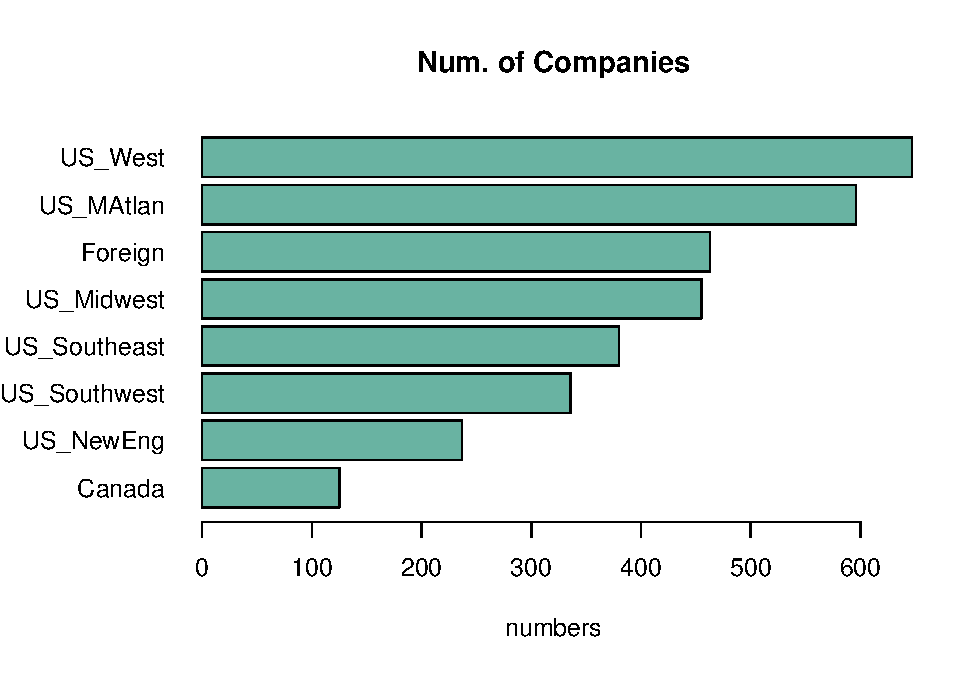
\includegraphics{final-project_files/figure-latex/unnamed-chunk-3-1.pdf}

\begin{verbatim}
## Clustering Gap statistic ["clusGap"] from call:
## clusGap(x = pca_data, FUNcluster = kmeans, K.max = 10, B = 50,     nstart = 25)
## B=50 simulated reference sets, k = 1..10; spaceH0="scaledPCA"
##  --> Number of clusters (method 'firstmax'): 2
##           logW    E.logW       gap      SE.sim
##  [1,] 9.644590 10.043184 0.3985936 0.006021833
##  [2,] 8.536762  9.813002 1.2762397 0.004550222
##  [3,] 8.388342  9.659794 1.2714519 0.004826090
##  [4,] 8.182432  9.527089 1.3446568 0.004066272
##  [5,] 8.099261  9.468178 1.3689172 0.003575720
##  [6,] 8.037787  9.415703 1.3779166 0.003779123
##  [7,] 8.002525  9.374597 1.3720725 0.003732857
##  [8,] 7.938119  9.337007 1.3988876 0.003660611
##  [9,] 7.935329  9.305535 1.3702058 0.003836592
## [10,] 7.871664  9.282829 1.4111650 0.003597734
\end{verbatim}

\includegraphics{final-project_files/figure-latex/unnamed-chunk-3-2.pdf}

\begin{verbatim}
##   cluster audit_fees_bc total_fees_bc market_cap_bc market_fee_ratio assets_log
## 1       1      14.32256      14.45650      21.14994         6.693444   21.00806
## 2       2      14.68737      14.85035      22.20569         7.355343   22.41399
##   revenue_trans earnings_trans
## 1      17.67397      -18.21096
## 2      21.21975       19.28884
\end{verbatim}

\begin{verbatim}
##   audit_fees_bc total_fees_bc market_cap_bc market_fee_ratio assets_log
## 1      14.01025      14.26595      22.26620         8.000254   21.90575
## 2      13.31298      13.31298      18.78857         5.475583   19.59625
## 3      13.70766      13.70766      20.98602         7.278362   19.78954
## 4      13.98102      13.98568      19.59019         5.604515   19.08812
## 5      11.46850      11.60027      20.21906         8.618788   20.03306
## 6      13.88246      13.94147      22.14374         8.202271   21.59282
##   revenue_trans earnings_trans cluster
## 1      20.91361      -18.43784       1
## 2      19.42208      -16.02850       1
## 3      19.33714       18.36820       2
## 4      19.67223      -17.38389       1
## 5      19.62253       16.85774       2
## 6      20.61072       18.13880       2
\end{verbatim}

\includegraphics{final-project_files/figure-latex/unnamed-chunk-3-3.pdf}
\# Step 5. 用lasso (已删除) 和Random Forest兩個model,找出會影響audit
fee的因素有哪些 \#\# for gamlr, and many other fitting functions, \#\#
We need to create the specific numeric feature matrix.

\begin{verbatim}
## 
## Call:
## summary.resamples(object = res)
## 
## Models: lm, knn, rf, cart, gbm 
## Number of resamples: 5 
## 
## MAE 
##           Min.   1st Qu.    Median      Mean   3rd Qu.      Max. NA's
## lm   0.5049889 0.5068346 0.5080532 0.5121576 0.5114575 0.5294535    0
## knn  0.4205690 0.4635588 0.4675670 0.4582595 0.4676018 0.4720010    0
## rf   0.4114225 0.4171427 0.4316190 0.4300918 0.4393486 0.4509262    0
## cart 0.4933624 0.5004241 0.5030845 0.5106017 0.5238028 0.5323350    0
## gbm  0.4136215 0.4328178 0.4369544 0.4349007 0.4452694 0.4458407    0
## 
## RMSE 
##           Min.   1st Qu.    Median      Mean   3rd Qu.      Max. NA's
## lm   0.6253952 0.6315272 0.6469873 0.6450307 0.6599200 0.6613238    0
## knn  0.5484462 0.5955556 0.5999170 0.5937151 0.6026957 0.6219609    0
## rf   0.5282347 0.5341068 0.5550453 0.5529947 0.5695266 0.5780603    0
## cart 0.6390846 0.6445624 0.6511338 0.6568797 0.6683214 0.6812961    0
## gbm  0.5385957 0.5558394 0.5658609 0.5609128 0.5661814 0.5780868    0
## 
## Rsquared 
##           Min.   1st Qu.    Median      Mean   3rd Qu.      Max. NA's
## lm   0.6469066 0.6549945 0.6700879 0.6728906 0.6945568 0.6979074    0
## knn  0.7092139 0.7122944 0.7211761 0.7250139 0.7317719 0.7506130    0
## rf   0.7415333 0.7562186 0.7655223 0.7615361 0.7718857 0.7725205    0
## cart 0.6465570 0.6558793 0.6618142 0.6613535 0.6666816 0.6758354    0
## gbm  0.7319783 0.7426083 0.7520331 0.7527188 0.7646105 0.7723640    0
\end{verbatim}

\hypertarget{step-7.-k-fold-cross-validation}{%
\subsubsection{Step 7. K-fold
Cross-validation}\label{step-7.-k-fold-cross-validation}}

\hypertarget{problem-lm-knn-lasso-ux7684k-fold-cvux600eux9ebcux505a}{%
\subsection{Problem: lm, knn, lasso 的k-fold
CV怎麼做}\label{problem-lm-knn-lasso-ux7684k-fold-cvux600eux9ebcux505a}}

\hypertarget{syntax-in-hw-3}{%
\subsection{Syntax in HW 3}\label{syntax-in-hw-3}}

\hypertarget{k-fold-cross-validation-k-1-is-training-set-1-is-testing-set}{%
\subsection{K-fold Cross-validation: (k-1) is training set, 1 is testing
set}\label{k-fold-cross-validation-k-1-is-training-set-1-is-testing-set}}

\hypertarget{ux5f9eux6c92ux7576ux904etesting-setux7684-datasetux4e2dux6311ux4e00ux500bux4f86ux505atesting-set-ux525bux525bux505aux904etesting-set-ux7684ux90a3ux4efdux5247ux52a0ux56deux53bbux505atraining-set}{%
\subsection{從沒當過testing set的 dataset中挑一個來做testing set,
剛剛做過testing set 的那份則加回去做training
set}\label{ux5f9eux6c92ux7576ux904etesting-setux7684-datasetux4e2dux6311ux4e00ux500bux4f86ux505atesting-set-ux525bux525bux505aux904etesting-set-ux7684ux90a3ux4efdux5247ux52a0ux56deux53bbux505atraining-set}}

\hypertarget{repeat-the-step-until-every-set-ux90fdux7576ux904etesting-set-ux6703ux57f7ux884ckux6b21-ux5f97ux5230kux500b-validation-error}{%
\subsection{repeat the step until every set 都當過testing set \#\#
會執行k次, 得到k個 validation
error}\label{repeat-the-step-until-every-set-ux90fdux7576ux904etesting-set-ux6703ux57f7ux884ckux6b21-ux5f97ux5230kux500b-validation-error}}

\hypertarget{average-the-k-validation-error-then-we-can-know-which-model-is-better}{%
\subsection{Average the k validation error, then we can know which model
is
better}\label{average-the-k-validation-error-then-we-can-know-which-model-is-better}}

\begin{verbatim}
## 
## Call:
##  randomForest(formula = total_fees_bc ~ five_category_factor +      state_region + market_cap_bc + assets_log + revenue_trans +      earnings_trans, data = data_train, importance = TRUE) 
##                Type of random forest: regression
##                      Number of trees: 500
## No. of variables tried at each split: 2
## 
##           Mean of squared residuals: 0.2981164
##                     % Var explained: 76.22
\end{verbatim}

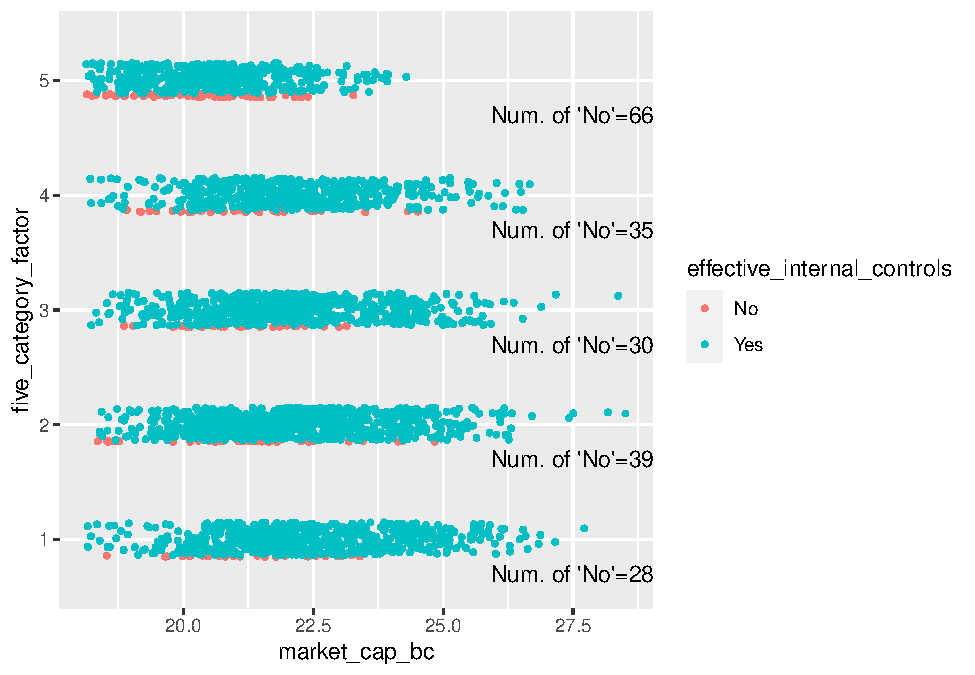
\includegraphics{final-project_files/figure-latex/unnamed-chunk-6-1.pdf}

\begin{verbatim}
## [1] 0.5844844
\end{verbatim}

\includegraphics{final-project_files/figure-latex/unnamed-chunk-6-2.pdf}
\includegraphics{final-project_files/figure-latex/unnamed-chunk-6-3.pdf}

\end{document}
